%%%%%%%%%%%%%%%%%%%%%%%%%%%%%%%%%%%%%%%%%
% Short Sectioned Assignment LaTeX Template Version 1.0 (5/5/12)
% This template has been downloaded from: http://www.LaTeXTemplates.com
% Original author:  Frits Wenneker (http://www.howtotex.com)
% License: CC BY-NC-SA 3.0 (http://creativecommons.org/licenses/by-nc-sa/3.0/)
%%%%%%%%%%%%%%%%%%%%%%%%%%%%%%%%%%%%%%%%%

%----------------------------------------------------------------------------------------
%	PACKAGES AND OTHER DOCUMENT CONFIGURATIONS
%----------------------------------------------------------------------------------------

\documentclass[paper=a4, fontsize=11pt]{scrartcl} % A4 paper and 11pt font size

% ---- Entrada y salida de texto -----

\usepackage[T1]{fontenc} % Use 8-bit encoding that has 256 glyphs
\usepackage[utf8]{inputenc}
\usepackage{fourier} % Use the Adobe Utopia font for the document - comment this line to return to the LaTeX default

% ---- Idioma --------

\usepackage[spanish, es-tabla]{babel} % Selecciona el español para palabras introducidas automáticamente, p.ej. "septiembre" en la fecha y especifica que se use la palabra Tabla en vez de Cuadro

% ---- Otros paquetes ----

\usepackage{url} % ,href} %para incluir URLs e hipervínculos dentro del texto (aunque hay que instalar href)
\usepackage{amsmath,amsfonts,amsthm} % Math packages
%\usepackage{graphics,graphicx, floatrow} %para incluir imágenes y notas en las imágenes
\usepackage{graphics,graphicx, float} %para incluir imágenes y colocarlas
\usepackage{epstopdf}
\usepackage[gen]{eurosym} %para incluir el símbolo del euro
\usepackage{cite} %para incluir citas del archivo <nombre>.bib
%\graphicspath{/images}

% Para hacer tablas comlejas
%\usepackage{multirow}
%\usepackage{threeparttable}

%\usepackage{sectsty} % Allows customizing section commands
%\allsectionsfont{\centering \normalfont\scshape} % Make all sections centered, the default font and small caps

\usepackage{fancyhdr} % Custom headers and footers
\pagestyle{fancyplain} % Makes all pages in the document conform to the custom headers and footers
\fancyhead{} % No page header - if you want one, create it in the same way as the footers below
\fancyfoot[L]{} % Empty left footer
\fancyfoot[C]{} % Empty center footer
\fancyfoot[R]{\thepage} % Page numbering for right footer
\renewcommand{\headrulewidth}{0pt} % Remove header underlines
\renewcommand{\footrulewidth}{0pt} % Remove footer underlines
\setlength{\headheight}{13.6pt} % Customize the height of the header

\numberwithin{equation}{section} % Number equations within sections (i.e. 1.1, 1.2, 2.1, 2.2 instead of 1, 2, 3, 4)
\numberwithin{figure}{section} % Number figures within sections (i.e. 1.1, 1.2, 2.1, 2.2 instead of 1, 2, 3, 4)
\numberwithin{table}{section} % Number tables within sections (i.e. 1.1, 1.2, 2.1, 2.2 instead of 1, 2, 3, 4)

\setlength\parindent{0pt} % Removes all indentation from paragraphs - comment this line for an assignment with lots of text

\newcommand{\horrule}[1]{\rule{\linewidth}{#1}} % Create horizontal rule command with 1 argument of height


%----------------------------------------------------------------------------------------
%	TÍTULO Y DATOS DEL ALUMNO
%----------------------------------------------------------------------------------------

\title{
\normalfont \normalsize
\textsc{\textbf{Ingeniería de Servidores (2016-2017)} \\ Grado en Ingeniería Informática \\ Universidad de Granada} \\ [25pt] % Your university, school and/or department name(s)
\horrule{0.5pt} \\[0.4cm] % Thin top horizontal rule
\huge Memoria Práctica 3 \\ % The assignment title
\horrule{2pt} \\[0.5cm] % Thick bottom horizontal rule
}

\author{Adrián Morente Gabaldón} % Nombre y apellidos

\date{\normalsize\today} % Incluye la fecha actual

%----------------------------------------------------------------------------------------
% DOCUMENTO
%----------------------------------------------------------------------------------------

\begin{document}

\maketitle % Muestra el Título

\newpage %inserta un salto de página

\tableofcontents % para generar el índice de contenidos

\newpage

\listoffigures

\listoftables

\newpage


\section{a) ¿Qué archivo le permite ver qué programas se han instalado con el gestor de paquetes? b) ¿Qué significan las terminaciones \emph{1.gz} o \emph{2.gz} de los archivos en ese directorio?}

	\subsection{Consulta de los paquetes instalados con APT}
	Como comentamos siempre en clase de prácticas, una de las cosas que tenemos que revisar como administradores de sistemas son los archivos \emph{.log}, los cuales contienen frecuentemente información relevante sobre paquetes instalados o servicios ofrecidos. En este caso, podemos consultar los paquetes instalados de APT a través del archivo ubicado en \emph{/var/log/apt/history.log}. En la misma carpeta podemos encontrar también el archivo \emph{term.log}, que contiene los resultados de instalación, consulta y borrado de paquetes realizados por APT. \\
	En la siguiente imagen, vemos el contenido del directorio mencionado, e imprimimos el contenido del fichero \emph{history.log} incluido en tal sitio; ya que en él encontramos la información pedida por el enunciado:
	\begin{figure}[H]
		\centering
		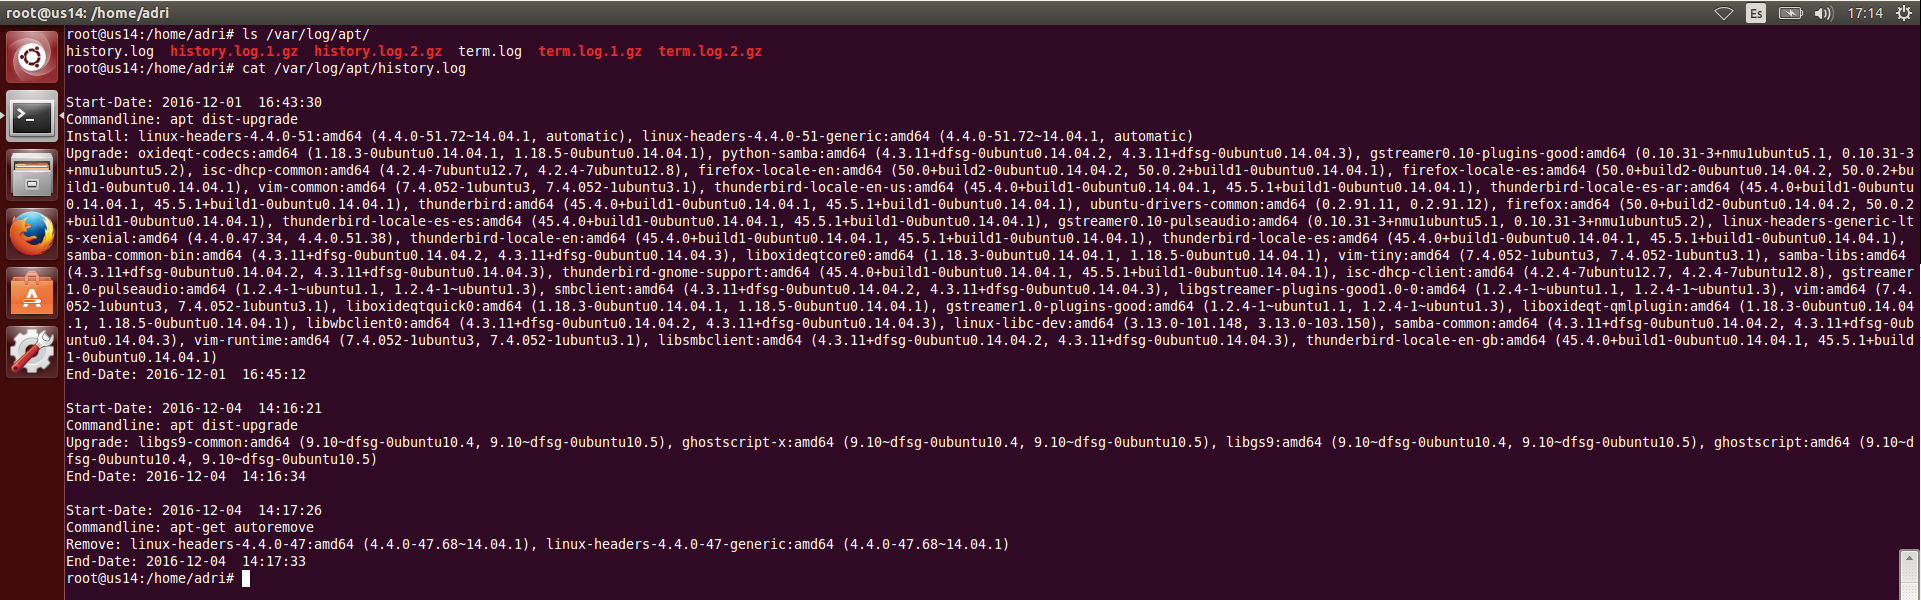
\includegraphics[scale=0.3]{apt-history}
		\caption{Consulta de los paquetes instalados con APT en el directorio /var/log/apt. - Adrián Morente Gabaldón [04/12/2016]}
		\label{figura1}
	\end{figure}
	En cuanto a la extensión del contenido del archivo, que vemos que es muy reducida, hablaremos de ello en el siguiente apartado del ejercicio. En este caso, podemos ver en los apartados \textbf{Commandline: apt ...} que las últimas acciones que realicé en la administración de Ubuntu Server fueron las actualizaciones del sistema, con los consiguientes borrados automáticos de programas y/o paquetes innecesarios. \\
	A continuación, vemos parte del contenido del archivo \emph{term.log}, que concuerda con las actualizaciones y borrados realizados arriba, ya que aquí se recogen los resultados de dichas acciones:
	\begin{figure}[H]
		\centering
		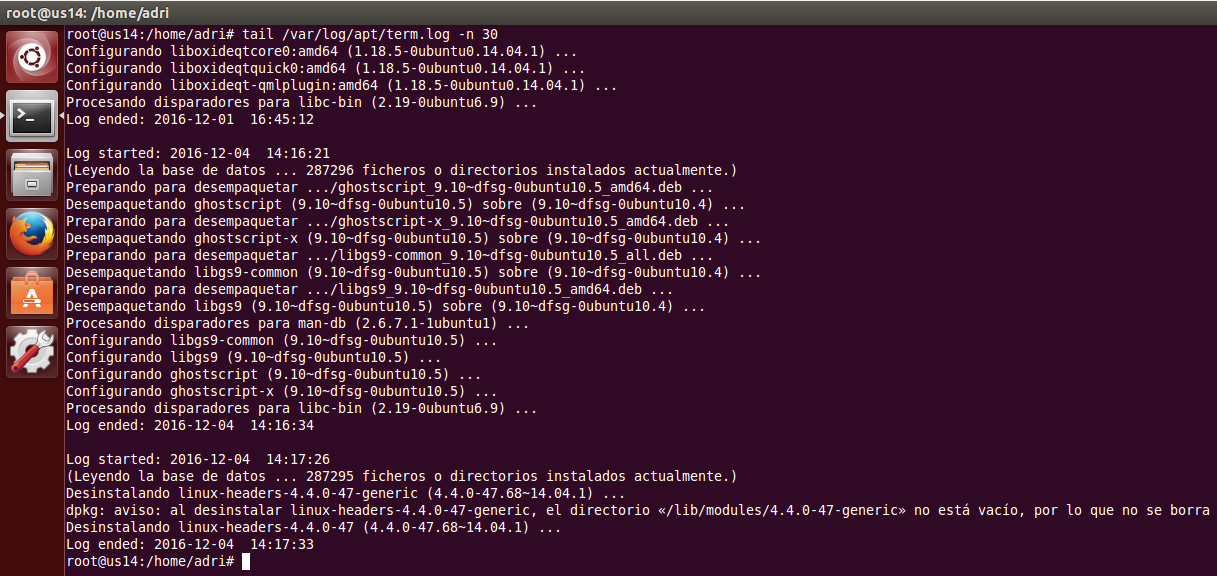
\includegraphics[scale=0.4]{apt-term}
		\caption{Contenido del archivo \emph{term.log} y los resultados de la ejecución de APT. - Adrián Morente Gabaldón [04/12/2016]}
		\label{figura2}
	\end{figure}

	\subsection{Archivos \emph{1.gz} y \emph{2.gz} del gestor APT}
	Como podemos ver en los manuales oficiales de GNU \cite{gzip}, los archivos con extensión \emph{.gz} son archivos comprimidos manejados por sistemas operativos basados en Unix. El gestor de paquetes APT deposita el historial y los resultados de sus ejecuciones en los archivos \emph{history.log} y \emph{term.log} respectivamente, como hemos visto antes; pero conforme esos archivos comienzan a tener un tamaño elevado, el sistema decide comprimir su contenido para ahorrar espacio. Por ejemplo, para el archivo \emph{history.log}, comprimirá todo su contenido en un nuevo archivo \emph{history.log.X.gz} siendo X el número de veces que se ha realizado esta acción. Es decir, si el sistema ha hecho esto tres veces, tendremos los tres archivos \emph{history.log.1.gz}, \emph{history.log.2.gz} y \emph{history.log.3.gz}; siendo siempre más reciente aquel con numeración menor.

\section{¿Qué archivo ha de modificar para programar una tarea? Escriba la línea necesaria para ejecutar una vez al día una copia del directorio ~/codigo a ~/seguridad/\$fecha donde \$ fecha es la fecha actual (puede usar el comando date).}
Para informarnos sobre el uso de \emph{cron} (herramienta ya utilizada en la asignatura de Sistemas Operativos) podemos utilizar el manual a través de la línea de comandos, aunque en mi caso utilizaré también la documentación oficial de Oracle al respecto \cite{cron}, que en mi caso es más ilustrativa para el uso de dicha herramienta. \\
Como vemos en la web, el archivo modificado al programar una tarea es \textbf{/var/spool/cron/crontabs}, pero es preferible no modificarlo directamente; sino hacerlo a través de la ejecución de la herramienta \emph{crontab}, como haremos en este caso práctico.
Para empezar, crearemos el script \emph{script\_seguridad.sh} que después ejecutaremos periódicamente, que tendrá el siguiente contenido:
\begin{verbatim}
	#!/bin/bash
	  #guarda la fecha actual en la variable
	date=$(date '+%Y%m%d_%H%M%S')
	  #si no existe, crea el directorio (primera vez)
	mkdir -p /seguridad/$date_time
	  #copia los archivos de /codigo a /seguridad/fecha
	cp -r ~/codigo/* ~/seguridad/$date_time
\end{verbatim}
A continuación, daremos permiso de ejecución al script (\emph{chmod u+x script\_seguridad.sh}) y crearemos varios ficheros de texto plano en el directorio \emph{~/codigo} con el contenido de prueba que queramos. \\
Antes de programar el archivo, volvamos a mirar la documentación de Oracle para ``refrescar la memoria'' en cuanto a la sintaxis de éstos \cite{cron-sintaxis}; y veremos que el orden de sus parámetros es:
\begin{verbatim}
<minuto> <hora> <día_mes> <mes> <día_semana> <comandos>
\end{verbatim}
Para terminar, crearemos el archivo \emph{cron} pero tal y como hemos dicho antes: sin acceder al fichero directamente sino a través de la herramienta \emph{crontab}. Como queremos que se ejecute una vez al día, podemos fijar que sus parámetros de ejecución sean siempre a las 5 de la tarde, lo cual sería de la siguiente forma:
\begin{lstlisting}[language=bash]
	crontab -e {0 17 * * * ~./script_seguridad.sh}
\end{lstlisting}

\section{Pruebe a ejecutar el comando, conectar un dispositivo USB y vuelva a ejecutar el comando. Copie y pegue la salida del comando. (considere usar dmesg | tail). Comente qué observa en la información mostrada.}
Como sabemos, el comando \emph{dmesg} puede ser muy útil para detectar problemas o cambios en el hardware conectado al kernel de un sistema; su uso es sencillo y da pie a muchas opciones (apenas usadas), según vemos en el manual del proyecto \emph{Linux Information Project} \cite{dmesg}. \\
Pasemos a ejecutar el comando \emph{dmesg | tail} para mostrar parte de esta información, y procedemos a insertar un pendrive USB en el ordenador, que seleccionamos a través del menú ``Dispositivos'' de la máquina virtual en VirtualBox de forma que el sistema virtual lo reconozca. Hecho esto, nos encontraremos con la siguiente imagen, en la que podemos ver cómo el kernel pasa a detectar el pendrive insertado, dándonos información del tipo de dispositivo (\emph{USB DISK 2.0}), el tamaño total (16GiB, 14.9GiB utilizables, en mi caso), el tamaño de cada bloque de datos en bytes (512B), y el modo de protección de escritura de datos (desactivado, ahora mismo) entre otros.
\begin{figure}[H]
	\centering
	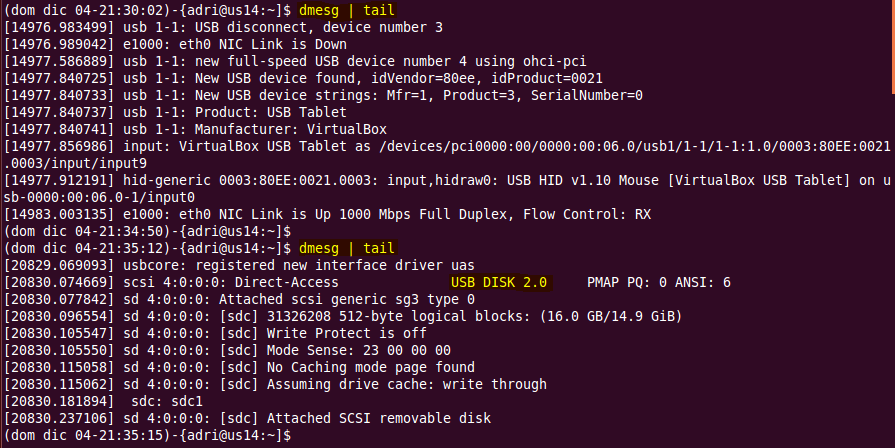
\includegraphics[scale=0.5]{dmesg}
	\caption{Muestra de los resultados recopilados del kernel por \emph{dmesg}. - Adrián Morente Gabaldón [04/12/2016]}
	\label{figura3}
\end{figure}

\section{Ejecute el monitor de ``System performance'' y muestre el resultado. Incluya capturas de pantalla comentando la información que aparece.}
El monitor de rendimiento \emph{perfmon} es una herramienta potente para analizar todo el estado del sistema en Windows Server, y aunque veremos parte de la información que nos muestra, no la comentaremos toda por razones obvias de tiempo y objetividad de la pregunta; para la que nos situaremos en varios estados del sistema operativo: ejecutaremos dos análisis, uno con el sistema sin hacer \textit{casi} nada; y otro con el sistema reproduciendo audio a través de una conocida plataforma de vídeo en streaming mediante el navegador \emph{Chrome}. \\
Para empezar, nos plantearemos en el primer caso descrito; en el que el sistema operativo tan solo tendrá abierto (con sus correspondientes procesos de fondo) la aplicación \emph{perfmon}, de forma que obtengamos unos resultados livianos en el análisis. \\ Una vez ejecutado el comando \emph{perfmon} desde PowerShell, en el panel de la izquierda iniciaremos una monitorización de \textbf{System Performance} tal y como se especifica en el guión. Tras un minuto de espera al análisis, obtenemos lo siguiente (se muestra una parte del complejo análisis completo):
\begin{figure}[H]
	\centering
	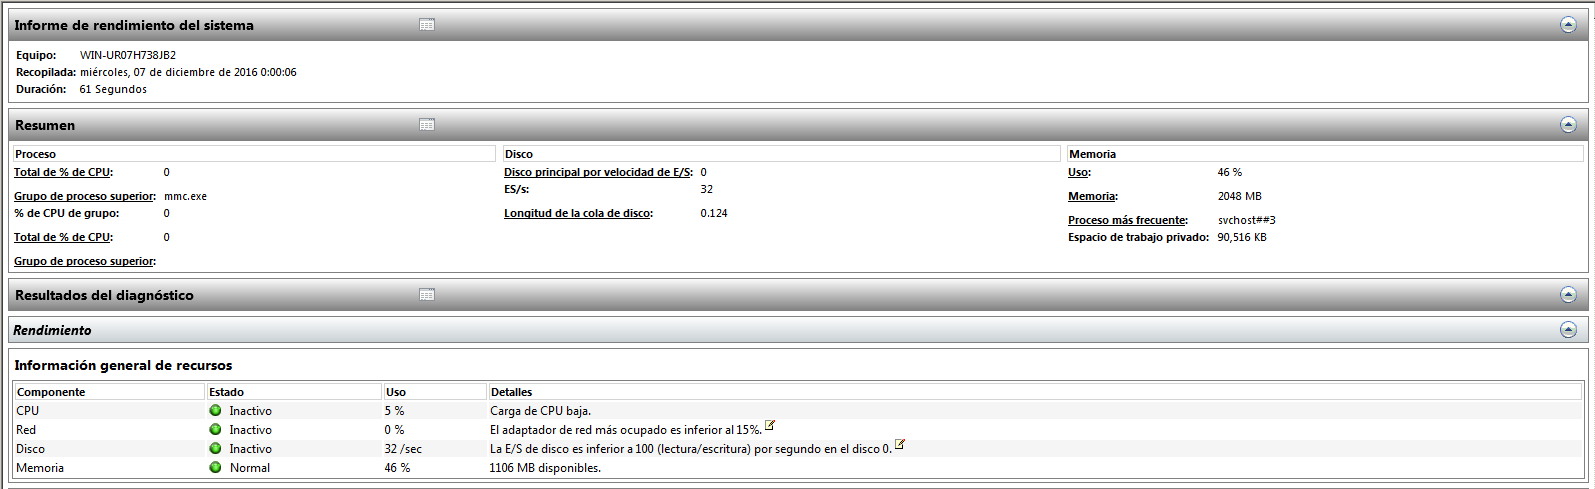
\includegraphics[scale=0.6]{perfmon-1}
	\caption{Primer informe de rendimiento del sistema con Perfmon. - Adrián Morente Gabaldón [06/12/2016]}
	\label{figura9}
\end{figure}
Fácilmente podemos ver que el consumo de la CPU es muy bajo y cercano al 0-5\%, ya que como hemos dicho el sistema está en estado \emph{idle}. Además, vemos que el consumo de memoria RAM también es muy ajustado (se ocupa el 46\% de los 2GiB que tenemos asignados a la máquina virtual). Veamos ahora otra captura con respecto al análisis de la memoria principal:
\begin{figure}[H]
	\centering
	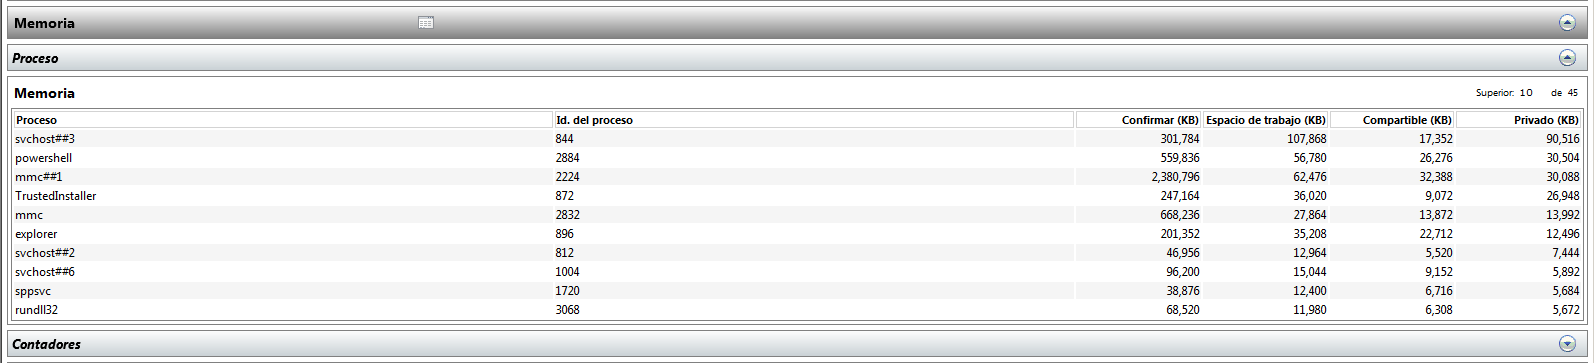
\includegraphics[scale=0.6]{perfmon-2}
	\caption{Informe de ocupación de la memoria principal con Perfmon. - Adrián Morente Gabaldón [06/12/2016]}
	\label{figura10}
\end{figure}
En esta última imagen vemos algunos de los procesos que se están ejecutando en primer o segundo plano en el sistema, junto con sus identificadores y el número de KB de memoria principal que ocupan. Si hiciéramos la suma, obviamente daríamos con el 46\% de los 2GiB de memoria antes mencionados. \\
Pasemos ahora al otro caso práctico en el que ocupamos parte de la memoria RAM con el navegador Chrome reproduciendo contenido multimedia. Iniciaremos un nuevo análisis de rendimiento de la misma forma antes descrita, obteniendo lo siguiente:
\begin{figure}[H]
	\centering
	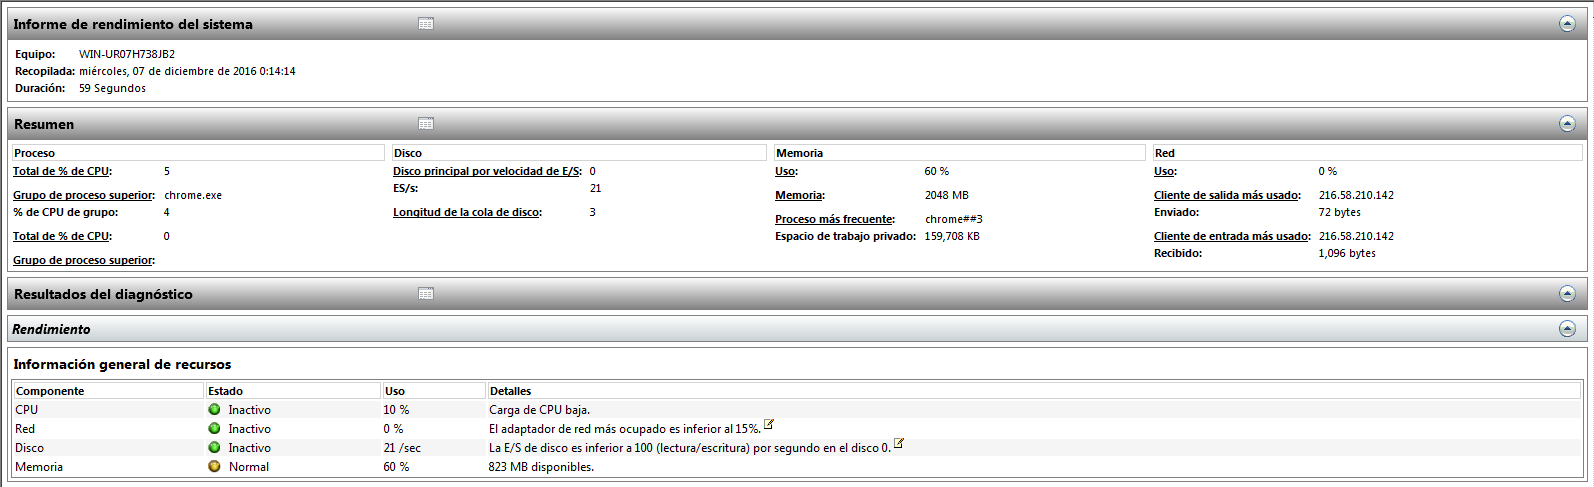
\includegraphics[scale=0.6]{perfmon-3}
	\caption{Segundo informe de rendimiento del sistema con Perfmon. - Adrián Morente Gabaldón [06/12/2016]}
	\label{figura11}
\end{figure}
Aunque seguimos sin hacer un gran trabajo de cómputo para la CPU, vemos como ha subido levemente su actividad, estando su carga comprendida ahora entre el 5\% y el 10\%


\section{Cree un recopilador de datos definido por el usuario (modo avanzado) que incluya tanto el contador de rendimiento como los datos de seguimiento: 1) Todos los referentes al procesador, al proceso y al servicio web. 2) Intervalo de muestra 15 segundos. 3) Almacene el resultado en el directorio Escritorio/logs. 4) Incluya las capturas de pantalla de cada paso.}

\section{Visite la web del proyecto y acceda a la demo que proporcionan (http://demo.munin-monitoring.org/) donde se muestra cómo monitorizan un servidor. Monitorice varios parámetros y haga capturas de pantalla de lo que está mostrando comentando qué observa.}
Según vemos en la documentación oficial de Munin, su nombre proviene de la mitología nórdica y significa \emph{memoria} \cite{munin-info}. Es una herramienta de monitorización en red, muy útil para examinar el rendimiento de los recursos y comprobar a qué se deben los \emph{bajones} puntuales de rendimiento. Además, sigue el estilo \textbf{``plug \& play''}, ya que con su instalación y muy poca configuración se puede empezar a funcionar rápidamente. \\
Si queremos instalarnos el servicio Munin en nuestra máquina con Ubuntu Server podemos seguir fácilmente la guía descrita en su web oficial \cite{munin-install}, en la que especifican que ambas partes (el modo ``master'' de administración y el modo ``nodo'') se encuentran en los repositorios oficiales de Debian (y por tanto de Ubuntu). \\
Pasemos a ver la versión ``demo'' de Munin en el enlace propuesto en el enunciado. Nada más acceder, nos encontramos con tres grupos:
\begin{itemize}
	\item \textbf{munin-monitoring.org}: será el que utilicemos en este caso, y a su vez comprende cuatro grupos:
	\begin{itemize}
		\item \emph{buildd.munin-monitoring.org}: dentro de éste, encontramos la clasificacion de cuatro recursos: \emph{disk} (datos del disco, datos de entrada-salida, latencia, etc), \emph{processes} (procesos de usuario, número de hebras, prioridad de éstas, etc), \emph{system} (uso de la CPU, uso de la tabla de descriptores de archivo, interrupciones, etc), y \emph{other} (que está en blanco). Comentaremos alguno de ellos más adelante.
		\item \emph{demo.munin-monitoring.org}: en este grupo encontramos muchos más recursos descritos, entre los que podemos ver detalladas las diferentes interfaces de red, memoria, disco, procesos e incluso contribuciones a \emph{GitHub} y mantenimiento de webs ofrecidas por nuestro servidor, entre otras. Sin embargo, no todos ellos están descritos y la mayoría aparecen en blanco. Comentaremos alguno más adelante.
		\item \emph{pi.munin-monitoring.org}: el recurso está en blanco, por lo que la demostración no nos deja profundizar más.
		\item \emph{www.munin-monitoring.org}:el recurso está en blanco, por lo que la demostración no nos deja profundizar más.
	\end{itemize}
	\item \textbf{vm}: solo comprende al recurso \textbf{bridge.vm} y está vacío. Entendemos que simula una conexión \emph{Bridge} entre recursos, pero la demostración no nos deja investigar más.
	\item \textbf{vpn}: solo comprende al recurso \textbf{nas.vpn} y está vacío. Entendemos que simula una conexión de red privada virtual (\emph{VPN}), pero la demostración no nos deja investigar más.
\end{itemize}
Para terminar, comentemos algunos de los recursos mencionados arriba. Empecemos con uno de los incluidos en el primer grupo (\emph{munin-monitoring.org}). A su vez, está clasificado dentro de la primera agrupación de éste: \emph{buildd.munin-monitoring.org}, en el apartado de ``procesos''. Se trata del \textbf{Fork rate}, que podemos traducir (según vimos en la asignatura de Sistemas Operativos) por el promedio de creación de procesos por segundo en el sistema. En el margen izquierdo contemplamos este promedio, mientras que en el margen horizontal inferior vemos su transcurso en el tiempo. La demostración también nos aporta la fecha y hora de dicha captura:
\begin{figure}[H]
	\centering
	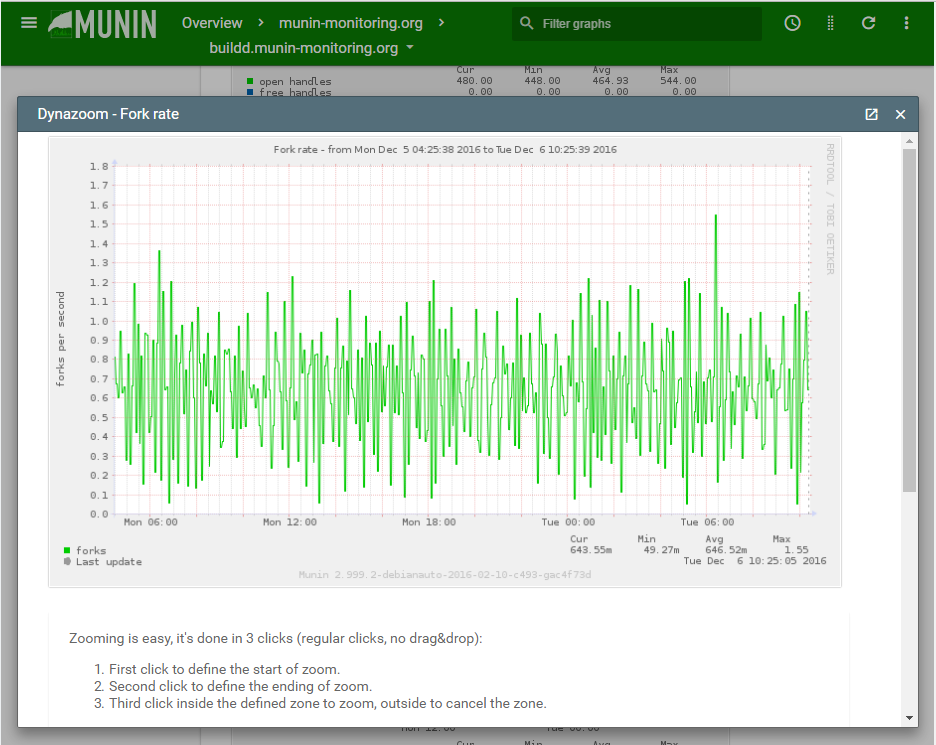
\includegraphics[scale=0.3]{munin-forkrate}
	\caption{Demostración del número de creación de procesos por segundo (Demostración de Munin). - Adrián Morente Gabaldón [06/12/2016]}
	\label{figura5}
\end{figure}
Y por último, veamos uno de los recursos incluidos en el grupo \emph{munin-monitoring.org} clasificado en \emph{demo.munin-monitoring.com}. Se trata de uno de los monitores de interfaces de red, y se trata de \textbf{Interface 1sec stats for eth0}. Este recurso vigila \textbf{cada segundo} la entrada/salida de datos (en bytes, en este caso) a través de la interfaz Ethernet del sistema. En el margen izquierdo vemos el número de K bytes manejados, y en el margen horizontal inferior su transcurso en el tiempo. También podemos ver la fecha y hora de dicho análisis:
\begin{figure}[H]
	\centering
	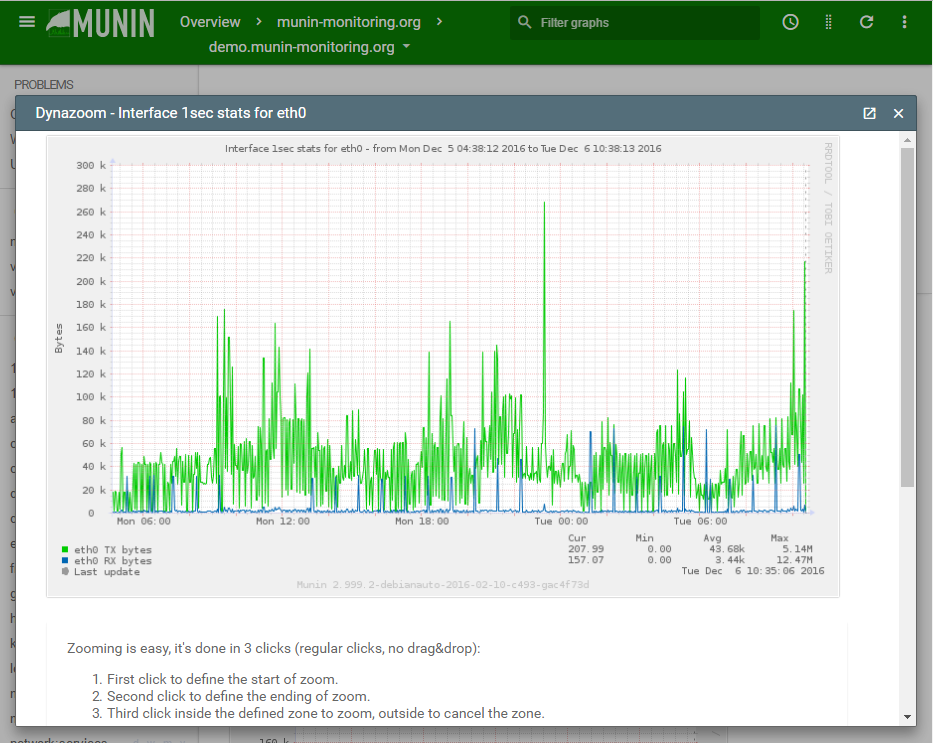
\includegraphics[scale=0.3]{munin-network}
	\caption{Demostración del manejo de bytes por segundo en la interfaz de red Ethernet (Demostración de Munin). - Adrián Morente Gabaldón [06/12/2016]}
	\label{figura6}
\end{figure}

\section{Escriba un breve resumen sobre alguno de los artículos donde se muestra el uso de strace o busque otro y coméntelo.}
En mi caso, haré un análisis del segundo artículo ofrecido en la práctica, proveniente del blog oficial de \textbf{SoftLayer, una compañía de IBM} \cite{softlayer-strace}. \\
Para empezar, plantean una descripción que nos sitúa en el marco de uso de la herramienta \emph{strace}, haciéndonos ver que su utilización va orientada a los administradores de sistemas (en este caso, nosotros); y que a través de su ejecución podemos analizar y corregir los errores de los servicios que ofrecemos mostrándonos las llamadas al sistema y las señales resultantes de la ejecución de dichos servicios. Gracias a esto, a través de los archivos \emph{.log} podemos ver cuál de los parámetros no están bien configurados o qué paquetes están fallando de alguna forma. \\
Para utilizar esta herramienta, solo tendremos que añadir el comando ``strace'' delante del comando o programa que queremos ejecutar, lo que provocará la impresión de las llamadas al sistema y las señales realizadas por la ejecución de éste. Cabe mencionar que deberemos tener permisos de usuario \emph{root} para su utilización. \\
Un caso de uso real en el que podemos ilustrar sobre la utilidad de \emph{strace} es a la hora de descubrir dónde están los archivos \emph{.log} de uno de los servicios que ofrece nuestro sistema. Por ejemplo, en el artículo estudiado se propone el siguiente ejemplo, que consiste en localizar los ficheros \emph{.log} correspondientes al servicio Apache, a partir de buscar los comandos \textbf{open} que tratan de abrirlos durante su ejecución:
\begin{lstlisting}[language=bash]
	strace -Ff -o output.txt -e open /etc/init.d/httpd restart
\end{lstlisting}
Esta línea de comandos se traduce, componente a componente, en lo siguiente:
\begin{itemize}
	\item \textbf{strace}: como ya sabemos, esto hará la máquina imprimir las llamadas al sistema;
	\item \textbf{-Ff}: esta opción fuerza a buscar los ficheros siguiendo todas las rutas y directorios;
	\item \textbf{-o output.txt}: esta opción redirigirá la salida al fichero pasado como parámetro, \emph{output.txt} en este caso;
	\item \textbf{-e open}: filtrará todas las llamadas al sistema que contengan la cadena pasada como parámetro; ya que queremos buscar la ruta de los archivos \emph{.log} que el sistema intenta abrir;
	\item \textbf{/etc/init.d/httpd restart}: esta orden ya la hemos usado en la práctica anterior, y sabemos que reinicia el servicio Apache; lo que provocará la búsqueda/apertura de los ficheros que buscamos.
\end{itemize}
Tras ejecutar dicha orden, abriremos el archivo filtrando por la palabra \textbf{log}, y obtendremos el siguiente contenido:
\begin{figure}[H]
	\centering
	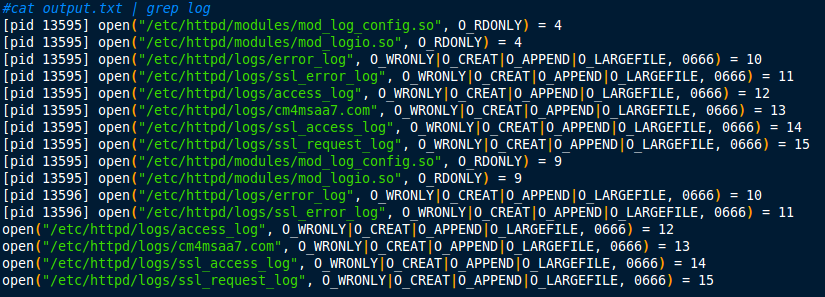
\includegraphics[scale=0.6]{strace}
	\caption{Salida filtrada de la ejecución de la orden con strace para la búsqueda de los \emph{logs} de Apache. - SoftLayer Blog [05/12/2016]}
	\label{figura4}
\end{figure}
Así solo veremos las líneas que pretenden abrir un fichero; y podemos observar que todas siguen el mismo patrón: 
\begin{verbatim}
	... open(...) = <número>
\end{verbatim}
El número asignado al final determina el número de operación de \emph{strace}, y será el identificador que utilice para trabajar con ese fichero. Por ejemplo, vemos que en una de las líneas intenta abrir el fichero \emph{/etc/httpd/logs/access\_log} y le asigna el identificador número 12; pues eso significará que estará utilizando ese fichero si por ejemplo encontramos una orden del tipo \textbf{read(12, ...<texto>) = XX}. Esta última se corresponde con una orden de lectura del fichero, que lo carga en memoria y le asigna tras el símbolo '=' el número de caracteres totales (XX genérico, en este caso). \\
Resumiendo, a través de la ejecución de \emph{strace} y del filtrado de sus mensajes de salida, podemos determinar dónde se encuentran los archivos correspondientes a cualquier fichero que busquemos. Además, la salida nos ilustra con números qué ficheros se abreen/leen y cuándo.


\section{Escriba un script en Python o PHP y analice su comportamiento usando el profiler presentado.}
En el enlace aportado por el enunciado, que dirige a la web oficial del lenguaje Python, encontramos tres tipos de profilers para dicho lenguaje:
\begin{itemize}
	\item \textbf{cProfile}: recomendado para la mayoría de usuarios, es escalable y apto para programas de ejecución extensa. Está escrito en C.
	\item \textbf{profile}: similar a \emph{cProfile} pero desarrollado en Python. A priori, su uso debería ser más sencillo para tareas simples.
	\item \textbf{hotshot}: se trata de un módulo experimental en C, el cual limita el tiempo de profiling a pesar de influir negativamente en el tiempo de procesamiento del resto de tareas. Está obsoleto y sin mantenimiento.	
\end{itemize}
Para este caso, utilizaremos el módulo \emph{cProfile}, el cual se puede incluir directamente en el código de la siguiente forma:
\begin{verbatim}
	import cProfile
	import re
	cProfile.run('re.compile("argumentos")')
\end{verbatim}
Sin embargo, esta opción me parece más liosa a nivel de código por lo que usaremos otra alternativa, que consistente en utilizar \emph{cProfile} a modo de script que ejecuta a otro. Es decir:
\begin{verbatim}
	python -m cProfile [-o fichero_salida] [-s orden_según parámetros] script.py
\end{verbatim}
Para empezar, veamos el código de nuestro simple script. Consiste en la definición de una clase con dos métodos simples. El tipo de objeto de la clase contendrá una cadena de texto y un número. El primer método imprime esta cadena carácter a carácter; mientras que el segundo método realiza unos cálculos algo más complejos con números para extender un poco el tiempo de ejecución del programa.
\begin{verbatim}
#!/usr/bin/python
# -*- coding: utf-8 -*-
"""script.py"""

class EjemploTexto:

  def __init__(self, texto, numero):
    self.texto = texto
    self.numero = numero

  def escribir(self):
    for i in self.texto:
    print("Dame una %s" % (i))

  def contar(self):
    for i in range(10000):
      for j in range(10000):
        self.numero += (i+j)

  def imprimir(self):
    print("Tengo un numero :) --> %s" % (self.numero))


ejemplo = EjemploTexto("PRACTICAS ISE", 81)

ejemplo.escribir()
ejemplo.imprimir()
ejemplo.contar()
ejemplo.imprimir()
\end{verbatim}
Ahora pasamos a ejecutar el script junto con el profiler, de la forma arriba mencionada, y obtendremos el siguiente resultado, que comentaremos a continuación:
\begin{figure}[H]
	\centering
	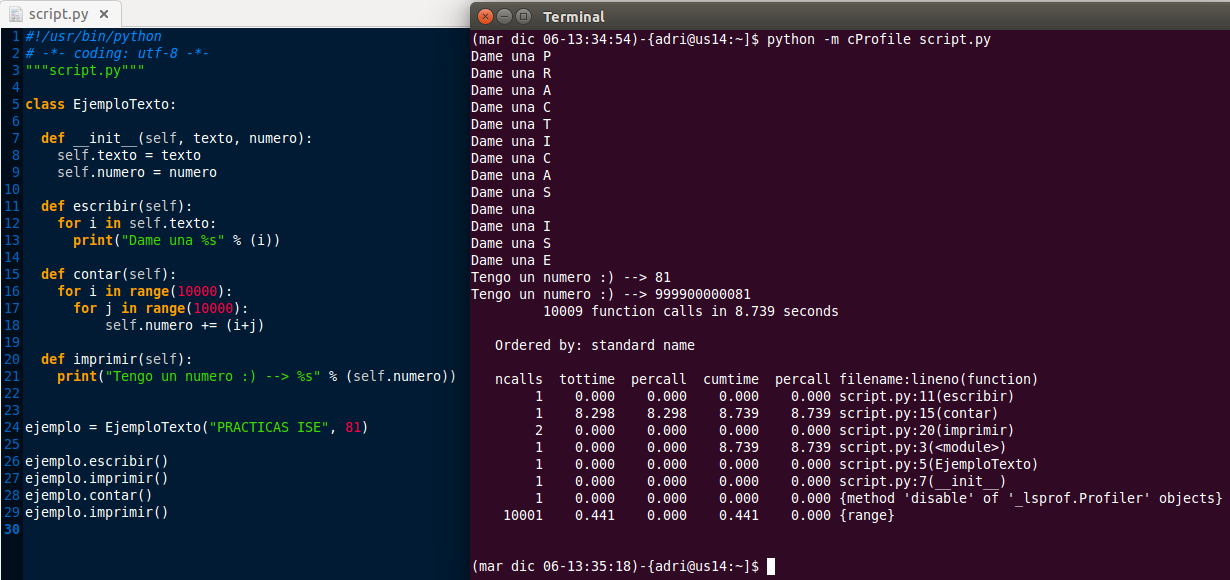
\includegraphics[scale=0.4]{python-cprofile}
	\caption{Ejecución del script de python junto con su profiler. - Adrián Morente Gabaldón [06/12/2016]}
	\label{figura7}
\end{figure}
Como podemos observar, el script tarda casi 9 segundos en ejecutarse (debido a los cálculos arriba mencionados), durante los que ejecuta 10.009 llamadas a funciones. En la tabla mostrada tras su ejecución, vemos el número de veces que se llama a cada una de éstas, siendo en todas 1 excepto en \emph{imprimir()} y \emph{range(...)}; esta última se llama tantas veces debido a los dos bucles anidados. Pasemos a ejecutar otra vez el script pero ordenando su salida de forma descendente con el tiempo de cómputo de cada una de las funciones. Esto lo haremos añadiendo \textbf{-s cumtime} al comando:
\begin{figure}[H]
	\centering
	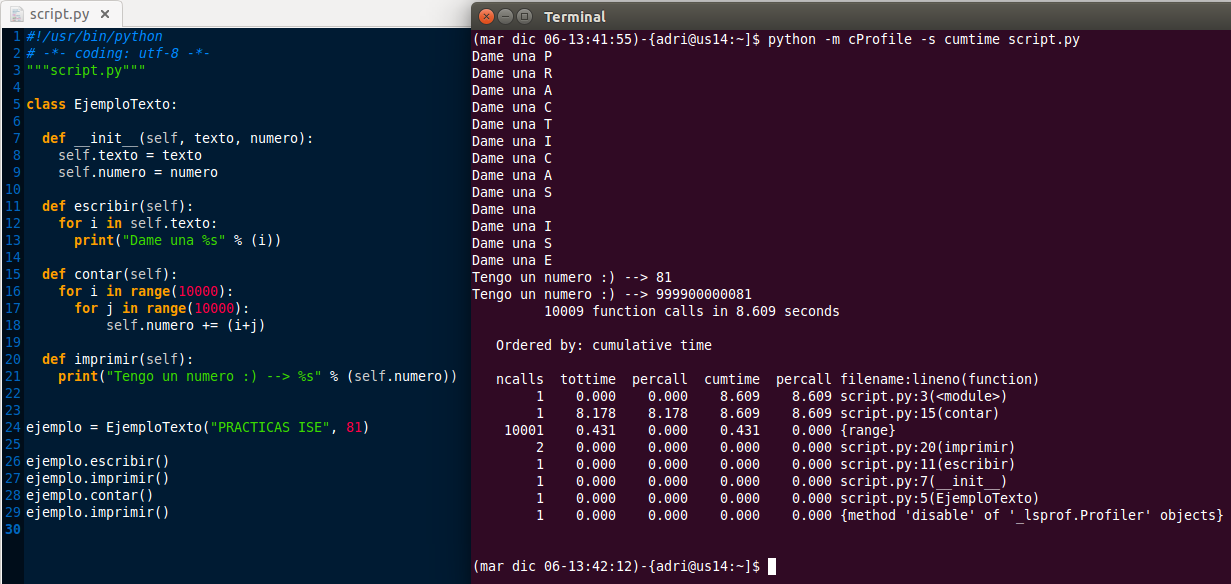
\includegraphics[scale=0.4]{python-cumtime}
	\caption{Ejecución del script de python junto con su profiler, ordenado según tiempo acumulativo de cada función. - Adrián Morente Gabaldón [06/12/2016]}
	\label{figura8}
\end{figure}
Como podemos apreciar, prácticamente todo el tiempo de cómputo está monopolizado por los cálculos del método \emph{contar()}, siendo casi despreciable en el resto de funciones.

\section{Acceda a la consola MySQL (o a través de phpMyAdmin) y muestre el resultado de mostrar el ``profile'' de una consulta (la creación de la BD y la consulta la puede hacer libremente).}


\bibliography{citas}
\bibliographystyle{plain}
\end{document}
